\documentclass[10pt,a4paper]{article}
\usepackage[utf8]{inputenc}
\usepackage[english]{babel}
\usepackage[T1]{fontenc}
\usepackage{amsmath}
\usepackage{amsfonts}
\usepackage{amssymb}
\usepackage{subcaption}
\usepackage{makeidx}
\usepackage{graphicx}
\usepackage{fourier}
\usepackage{listings}
\usepackage{color}
\usepackage{hyperref}
\usepackage[left=2cm,right=2cm,top=2cm,bottom=2cm]{geometry}
\author{Felipe Bruno, Vincent Noculak}
\title{Space Physics Project}

\begin{document}

\maketitle
\newpage
\tableofcontents
\newpage


\section{Introduction}

In this project we are going to study the space weather of the northern hemisphere of the earth at the 6. January 2011 between 18 and 24 o'clock universal time. We are going to do this by analysing the data of the ACE, SuperDARN, AMPERE, Ground-based magnetometers and All-Sky Cameras.

The phenomenons of space weather are mostly driven by the solar wind and its IMF (interplanetary magnetic field). The most important phenomenon of the interaction of the IMF and the terrestrial magnetic field is the Dungey cycle. This cycle can only happen when there is a southward IMF. It consists of the following steps which take approximately 12 hours to complete.

It begins with magnetic reconnection at the magnetopause between the in the opposite direction pointing magnetic field lines of the IMF and the earth. Due to the magnetic tension force and the solar wind, the reconnected field lines get dragged into the tail of the earth. The adding of magnetic flux to the tail compresses the plasma sheet. Now magnetic reconnection occurs in the tail. The reconnected and now again closed field lines of the earth return to the dayside where the cycle can begin anew.

\section{Instruments}

\subsection{All-Sky Camera}

In our project we are going to use the data of All-Sky cameras located in Svalbard at Ny Ålesund. These instruments are used to investigate the occurrence of auroras against time.
 Using a fish-eye lens, All-Sky cameras are able to take images of the whole sky. With an optical filter they can target the characteristic green and red light of the aurora. The cameras we are using have the filters at 5577 Å and 6300 Å. The cameras also include a photon counter to measure the brightness to the auroras. At \ref{a1} a typical keogram using an All-Sky Camera can be seen. While the colour gives the brightness, the x-axis gives the time and the y-axis gives the elevation. The diagram is made by taking the middle column of pixels in every photo the camera has taken and lining them up in the right time order.

\begin{figure}[h]
	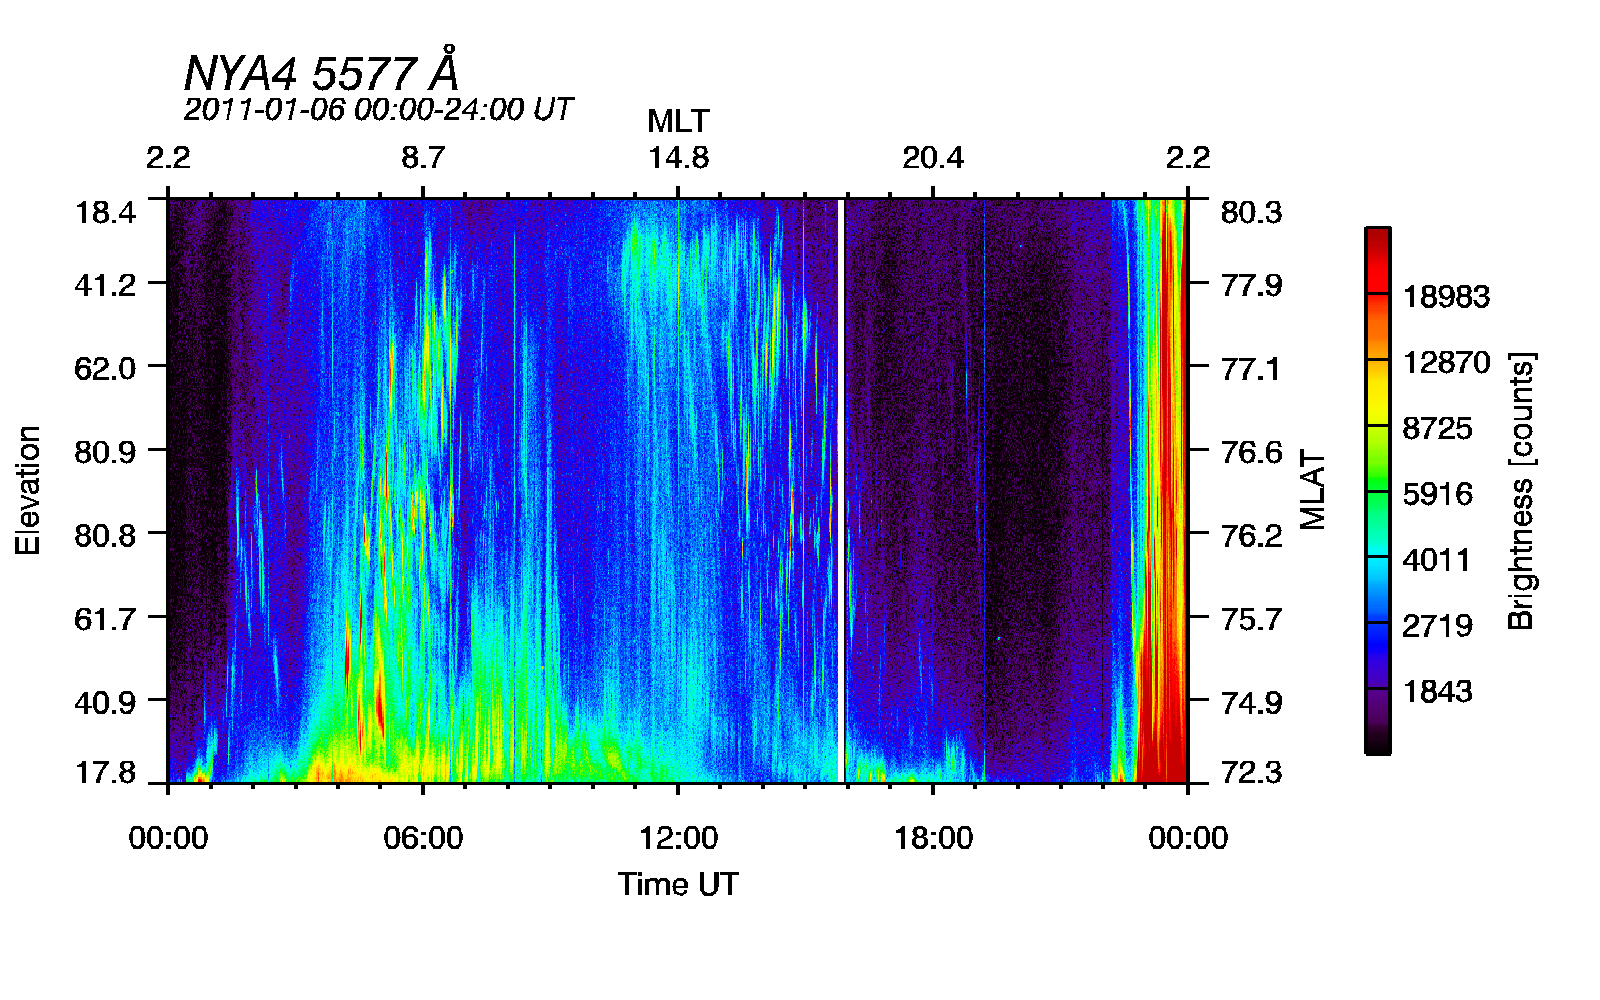
\includegraphics[scale = 0.20]{am-0024-5577.png}
	\centering
	\caption{Keogram of the All-Sky camera}
	\label{a1}
\end{figure}

\subsection{ACE}

The Advanced Composition Explorer, short ACE, is a satellite from NASA, which is among other things used to study the solar wind and its magnetic field. It orbits around the sun at the Lagrangian point $L_1$ so that it is always at a stable point between the earth and the sun, about $1.5 \cdot 10^6 km$ away from earth. 
One instrument of the satellite we are going to use is the SWEPAM (Solar Wind Electron, Proton and Alpha Monitor). With the instrument we can analysize the solar wind bulk speed to determine how much time it will need from the satellite to the earth. 
The other instrument we will use is the MAG (Magnetometer) to study the magnetic field of the solar wind.


\subsection{SuperDARN}

SuperDARN (Super Dual Auroral Radar Network) is a network of radars that consists of more than 30 low-power high frequency radars. It is used to measure plasma convection in the F-Region of the ionosphere at a high latitude. In \ref{s1} the area the radars of superDARN cover is shown. It can be seen that nearly the whole northern polar cap is covered by the radars. On Russia's side some ground at high latitude is not covered by the radars.
The radars are using the Doppler effect to measure convection. They send out electromagnetic waves at a specific frequency. In the Ionosphere the waves get reflected and have a Doppler shift due to movement of the plasma. From the change in frequency of the waves which return to the instruments, the velocity of the plasma can be determined.

\begin{figure}[h]
	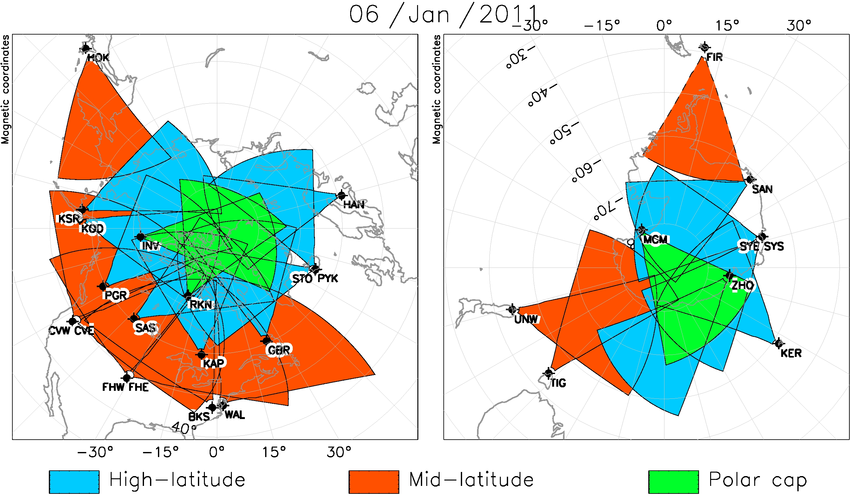
\includegraphics[scale = 1.5]{sd_1.png}
	\centering
	\caption{Covered area of the SuperDARN}
	\label{s1}
\end{figure}

\subsection{AMPERE}

AMPERE stands for "Active Magnetosphere and Planetary Electrodynamics Response Experiment". It uses the over 60  Iridium satellites which are orbiting earth to get information about the space weather. On the satellites are magnetometers to measure magnetic fields. From the measurement of those fields, field-aligned currents can be derived, using Amperes law. Thus the currents drawn in the diagrams belonging to AMPERE are not measured directly. Because of the amount of iridium satellites, the measurements are always covering the whole earth.

\subsection{Ground-based magnetometers}

In this project we are going to analyse the data on Ground-based magnetometers. Most of the magnetometers we are using are located in Norway, Sweden or Finland. A current always generates a magnetic field (Ampere's law). Hence by measuring the magnetic field on the ground, currents in the Ionosphere can be measured indirectly.

\section{Observations}

\subsection{All-Sky Camera}

The figure \ref{fig:sfig1} and \ref{fig:sfig2} show the keograms of the All-Sky Camera for the whole day on the 06.01.2011 for the green and red aurora. We look at the time span from 18 to 24 UT. On the first sight it can be seen that before 22 UT there is nearly no aurora, while after 22 UT there is a big onset of aurora. This timespan, 22-24 UT, will be discussed the most in this project.

Between 18 UT and 19 UT (figure \ref{fig:sfig3} and \ref{fig:sfig4}) it can be seen, that the the camera detects a lot of light at low latitudes. Most of this bright structure is outside of the range of the imager and is very stable in time. Hence it is difficult to decide if it is an aurora or a cloud. At 18:45 Ut there is a bright source at higher latitude, which moves southward for 10 minutes. By looking at the pictures the camera took separately and comparing the structure at both wavelengths, it can be seen that this is a cloud, which moves southward and then dissolves. 
In the timespan 19-22 UT, no auroral activity is happening in the area the All-sky camera observes.

 In figure \ref{fig:sfig5} and \ref{fig:sfig6} it can be seen, that ,starting with 22:20 UT, a long aurora forms at the western sky up to 82° geomagnetic latitude and moves southward down to 75° MLAT at 22:50 UT. This could be an auroral arcs, which usually appear during the growth phase of a substorm. During the end of that movement, starting from 22:45 UT, there is a large onset of aurora, which starts at low latitudes (72.3 MLAT), where at that time the aurora has travelled. This onset then moves very quickly to higher latitudes. At 23:28 the auroras are already at 80° MLAT and stay at latitudes this high up until 0:00 UT. During that movement, the auroras a very unstable, for example when they increase their intensity a lot at 23:10 UT, then get less intense and peak again from 23:25 to 23:33 UT. The last peak of onset of auroras then is from 23:50 to after 0:00 UT.
The biggest onset of green aurora is between 23:28 and 23:29 UT. In this time frame the green aurora covers nearly the whole sky, while the red is not as strong. The red aurora is especially strong between 23:03 and 23:09 UT.
The sudden strong increases of auroral activity starting from 22:45 UT are a sign of a starting expansion phase of a substorm.

 In the night of the 06.01.2011 it looks like there is a especially big substorm happening between 22:20 and 24:00 UT, which has three peeks in activity at 23:05 UT, 23:28 UT and between 23:50-24:00 UT.
We can see the growth phase of the substorm 22:20-22:50 UT, when the aurora, we described, moves in form of an auroral arc southward, due to dominating dayside reconnection and as a consequence an expanding polar cap. At 22:45 the expansion phase of the substorm starts. It has the typical characteristics of this phase, because the auroral arc suddenly brightens, moves poleward quickly and then already fills nearly the whole sky at 23:28 UT (figure \ref{i2}). In this phase, the auroras move from 77.5° MLAT at 23:20 UT to 81°-82.5° MLAT at 23:32 UT and stay at this latitude to after 24:00 UT. It happens that the intensity of auroral activity decreases between 23:05 and 23:20 UT and 23:45 and 23:50 UT, but we would not describe this time-spans as a recovery phase, because they last a very short time and are quickly followed by a big increase of auroral activity again. The real recovery phase of the substorm begins after 24:00 UT.   

\begin{figure}[h]
	\begin{subfigure}{.5\textwidth}
		\centering
		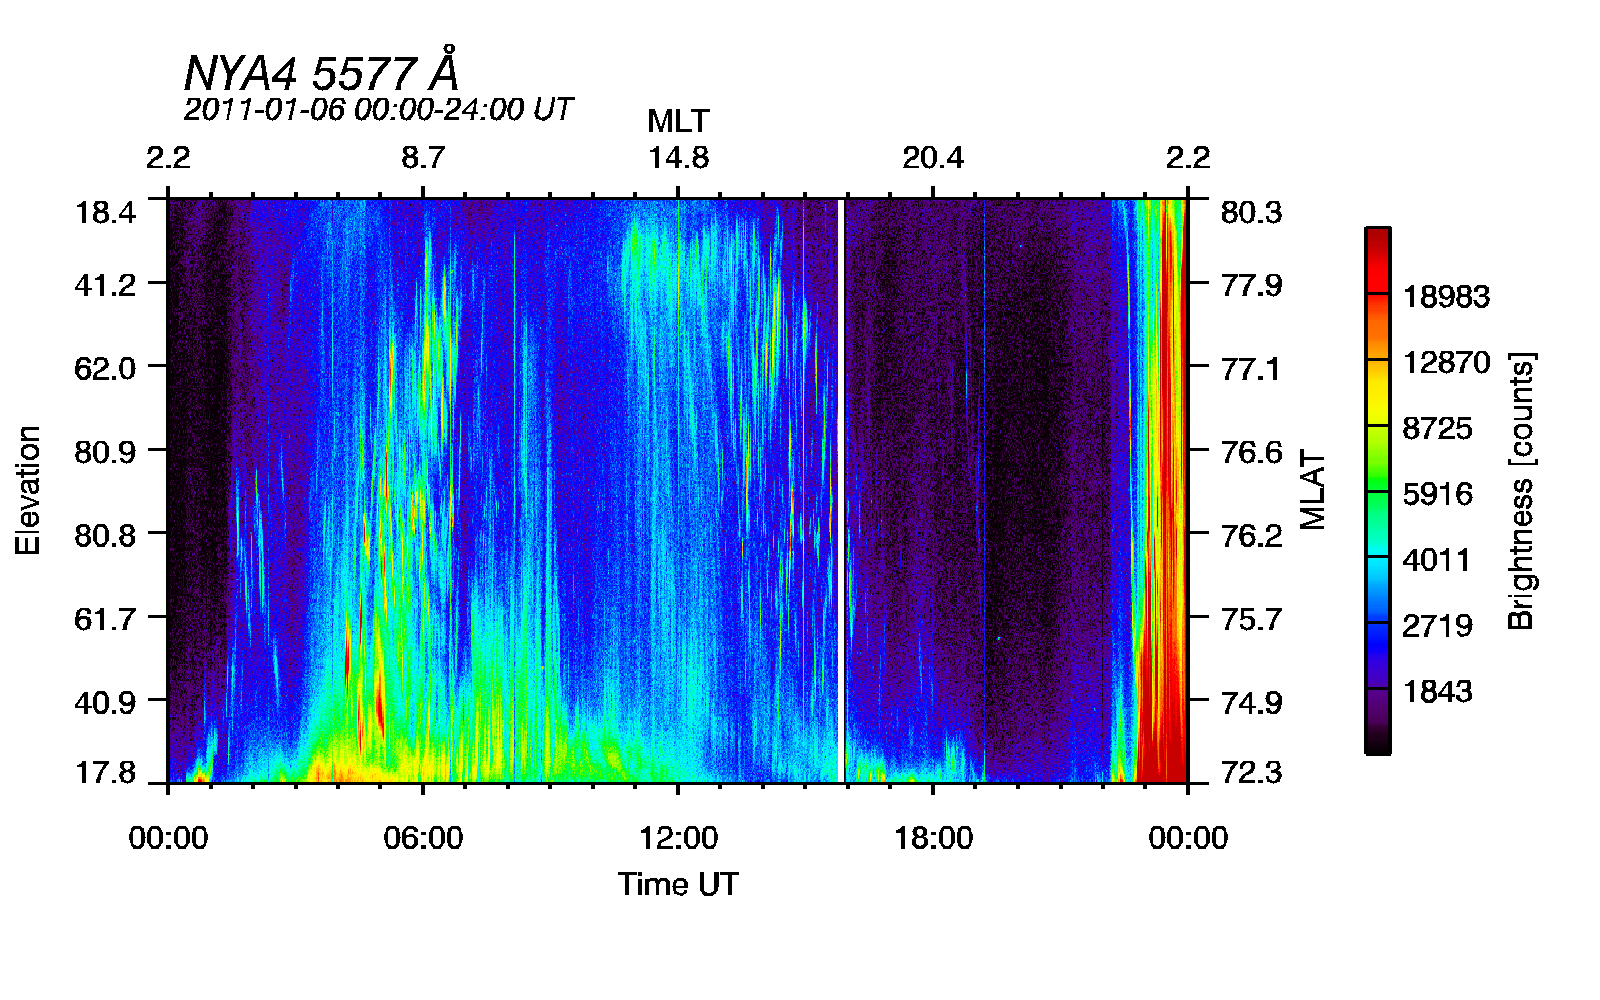
\includegraphics[width=.8\linewidth]{am-0024-5577.png}
		\caption{0-24 UT, 5577 Å}
		\label{fig:sfig1}
	\end{subfigure}
	\begin{subfigure}{.5\textwidth}
		\centering
		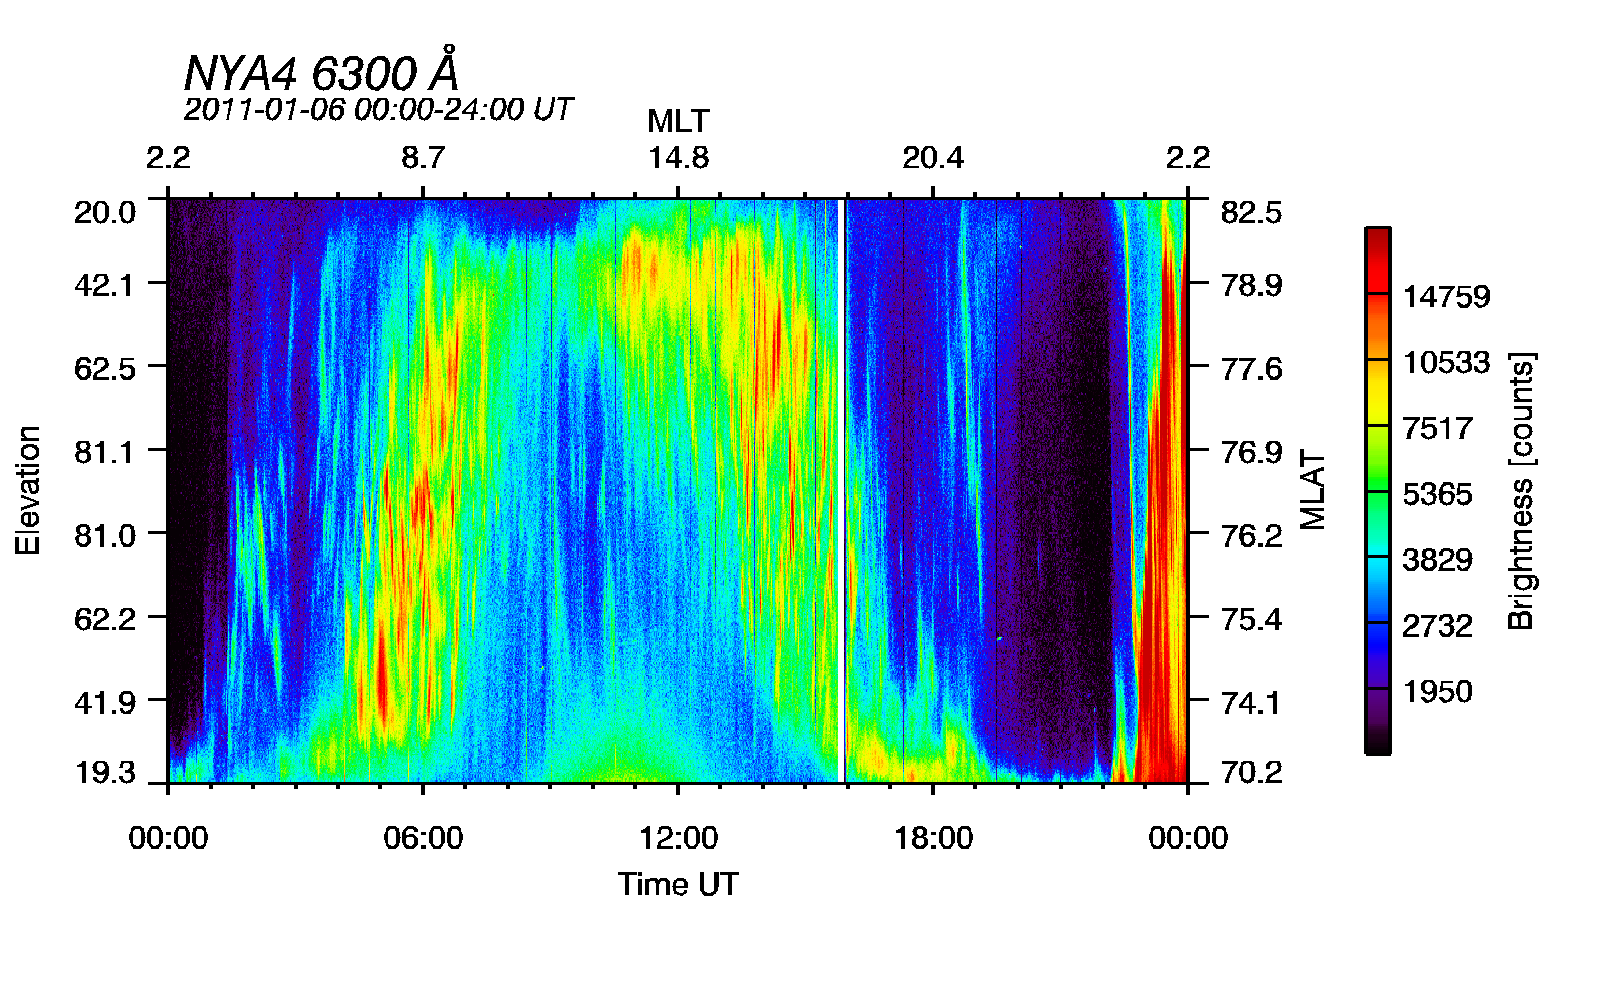
\includegraphics[width=.8\linewidth]{am-0024-6300.png}
		\caption{0-24 UT, 6300 Å}
		\label{fig:sfig2}
	\end{subfigure}
	\begin{subfigure}{.5\textwidth}
		\centering
		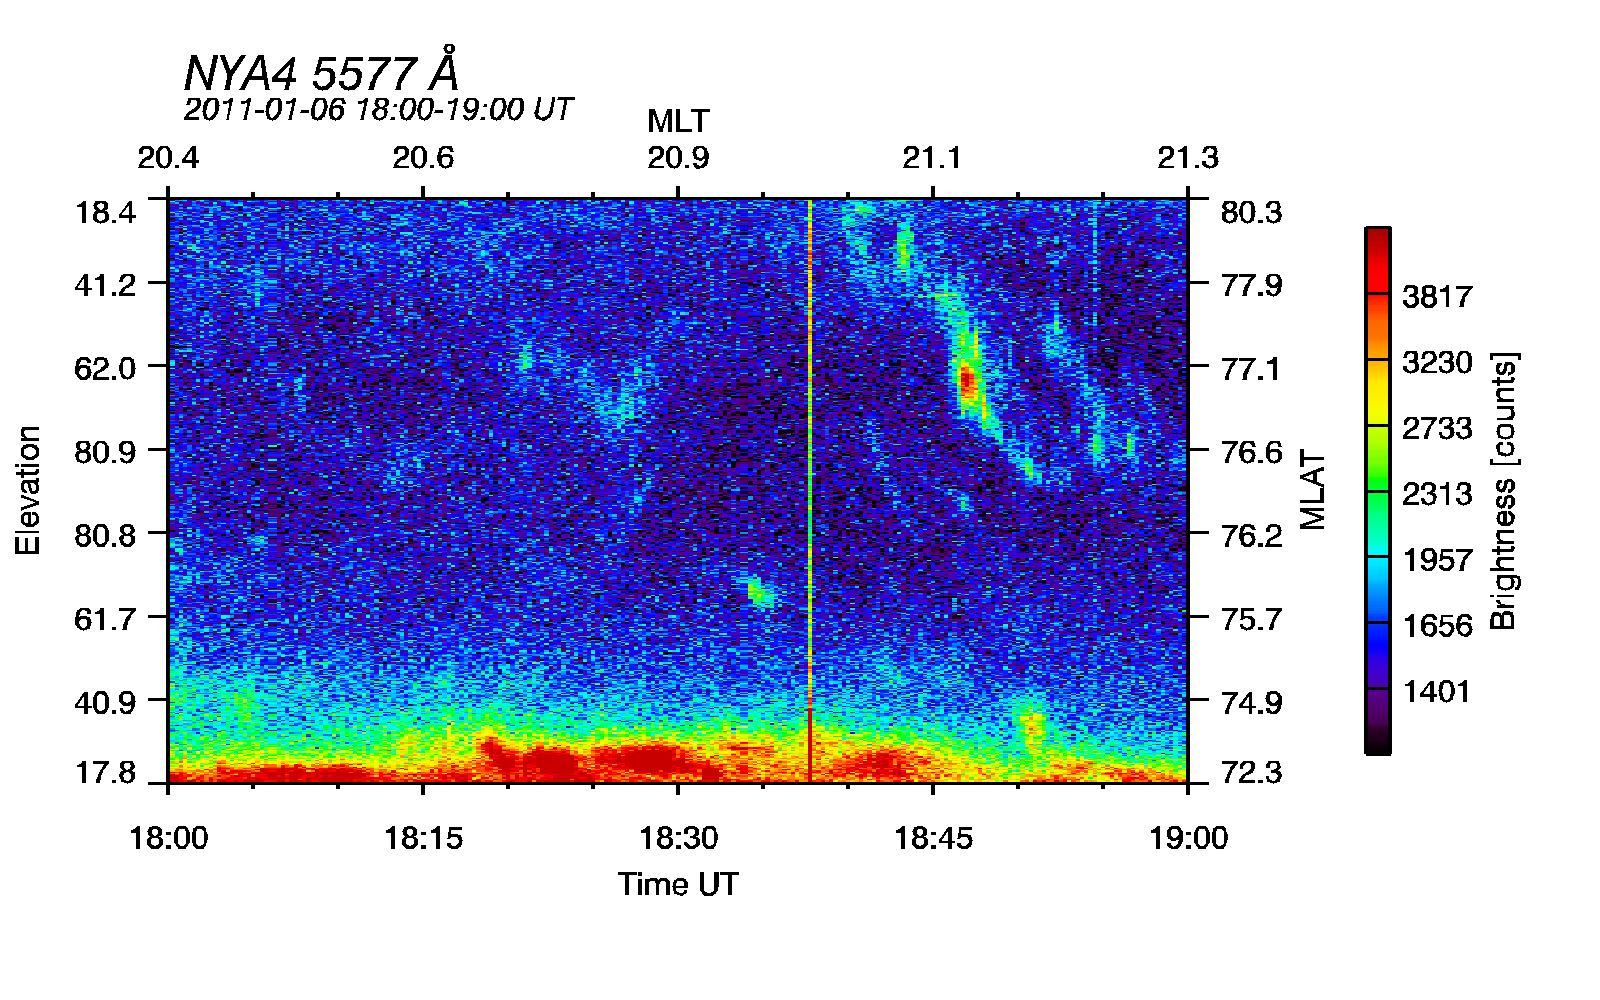
\includegraphics[width=.8\linewidth]{am-1819-5577.png}
		\caption{18-19 UT, 5577 Å}
		\label{fig:sfig3}
	\end{subfigure}
	\begin{subfigure}{.5\textwidth}
		\centering
		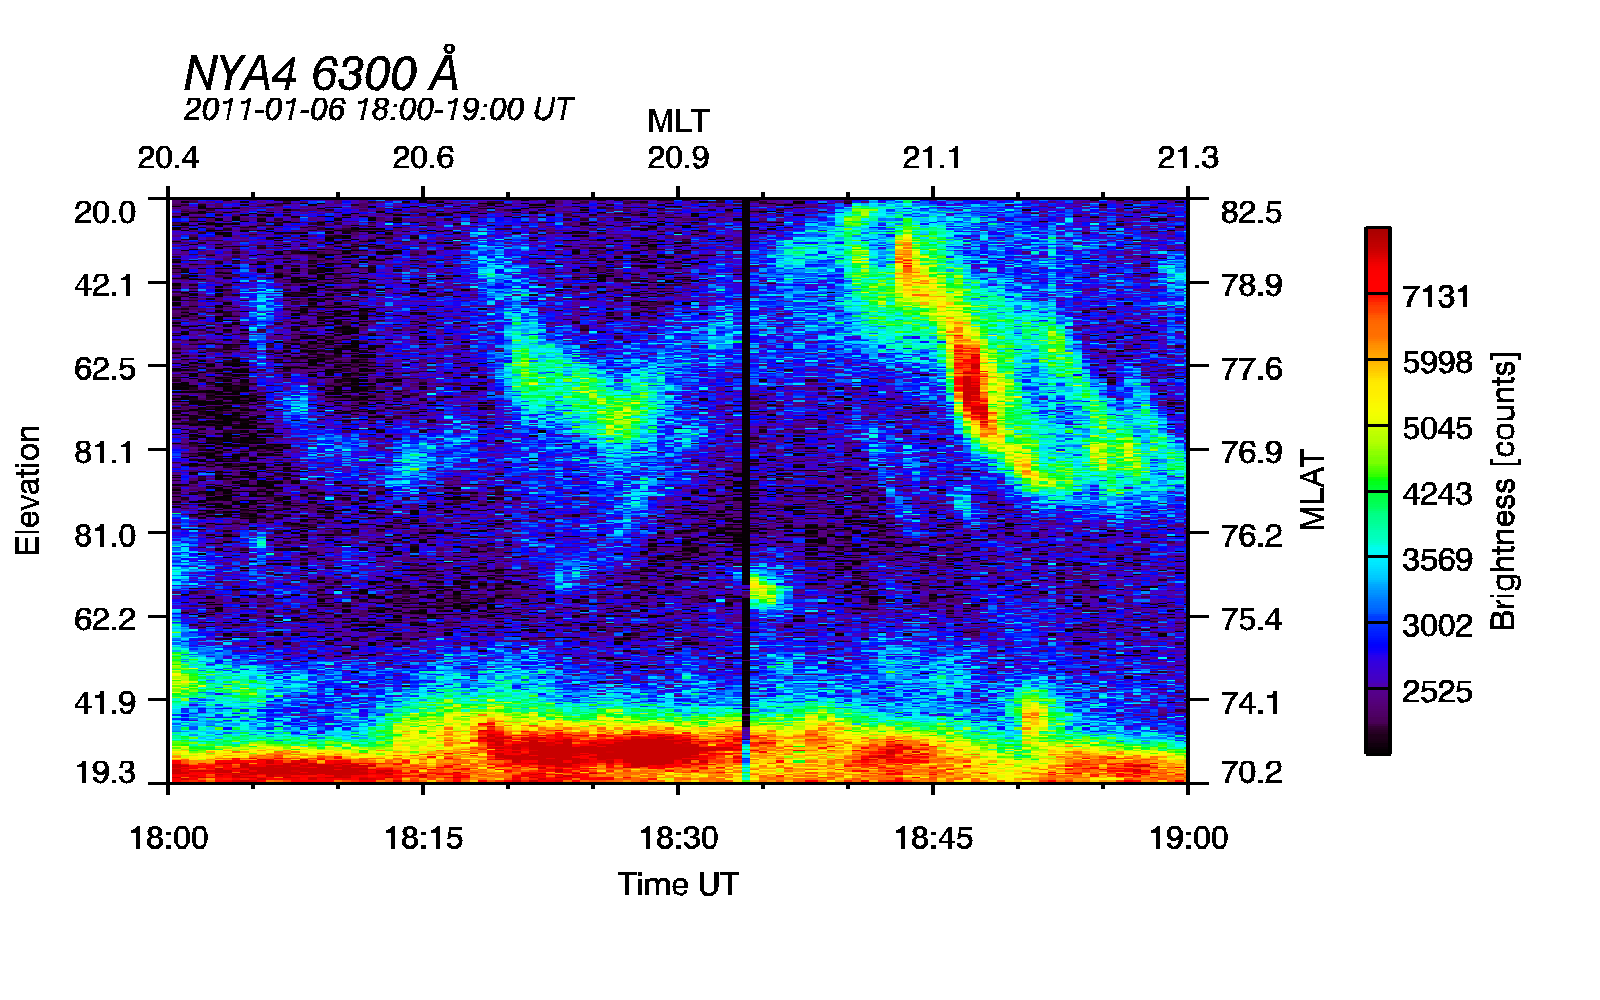
\includegraphics[width=.8\linewidth]{am-1819-6300.png}
		\caption{18-19 UT, 6300 Å}
		\label{fig:sfig4}
	\end{subfigure}
	\begin{subfigure}{.5\textwidth}
		\centering
		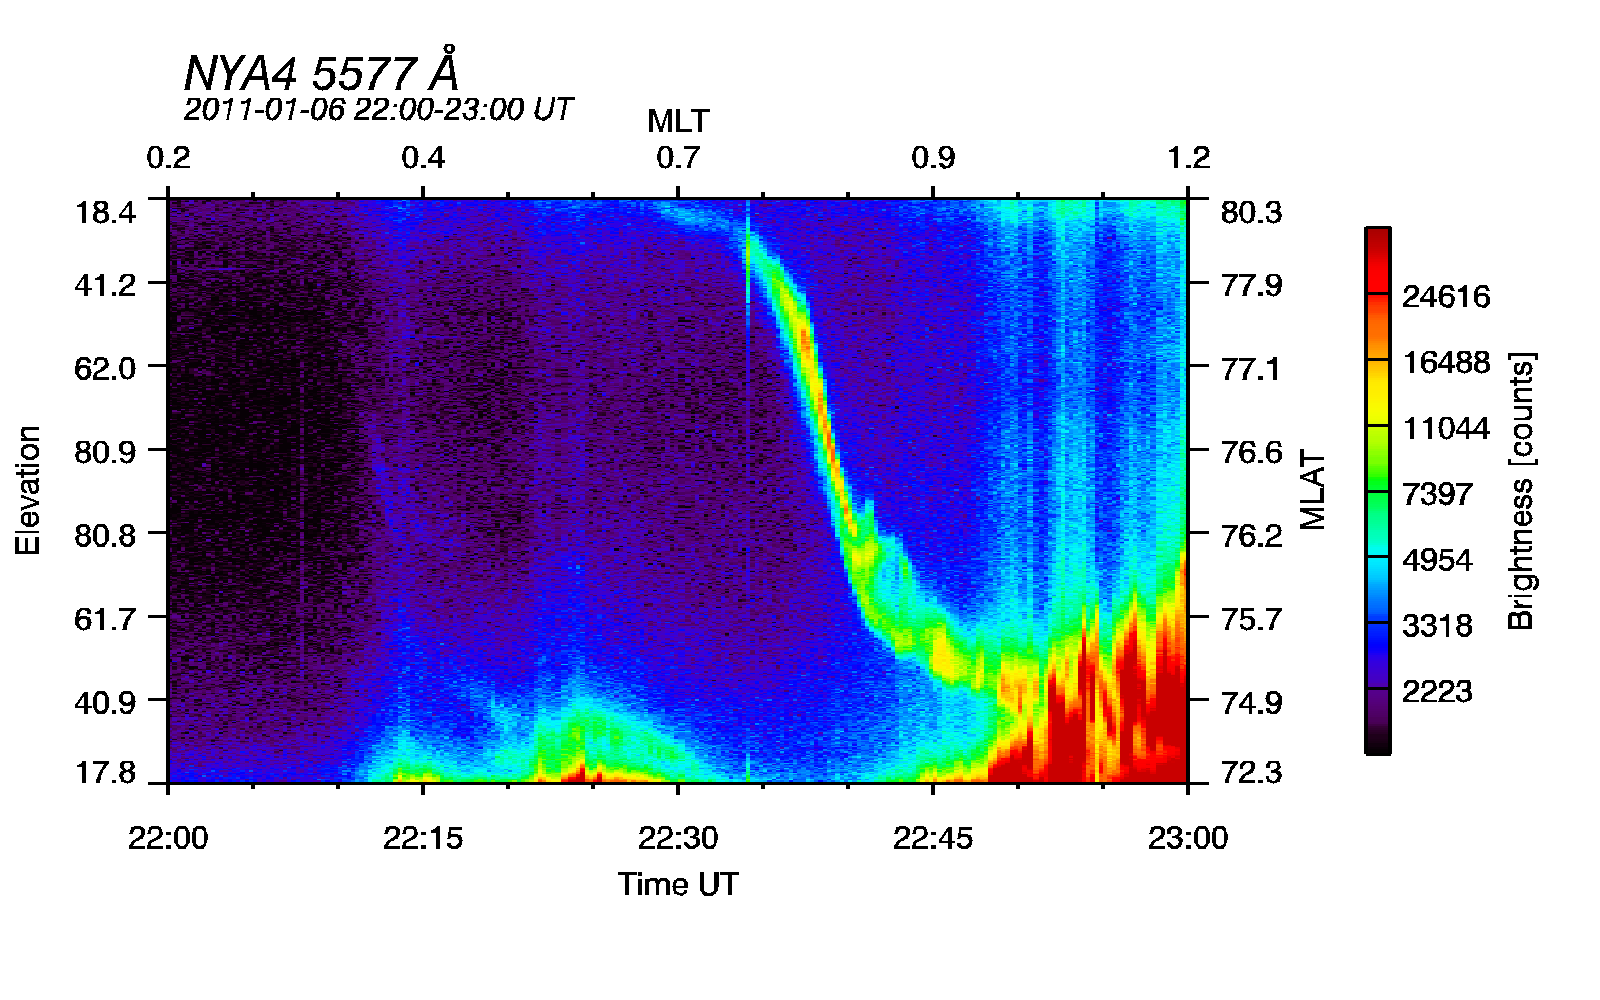
\includegraphics[width=.8\linewidth]{am-2223-5577.png}
		\caption{22-23 UT, 5577 Å}
		\label{fig:sfig5}
	\end{subfigure}
	\begin{subfigure}{.5\textwidth}
		\centering
		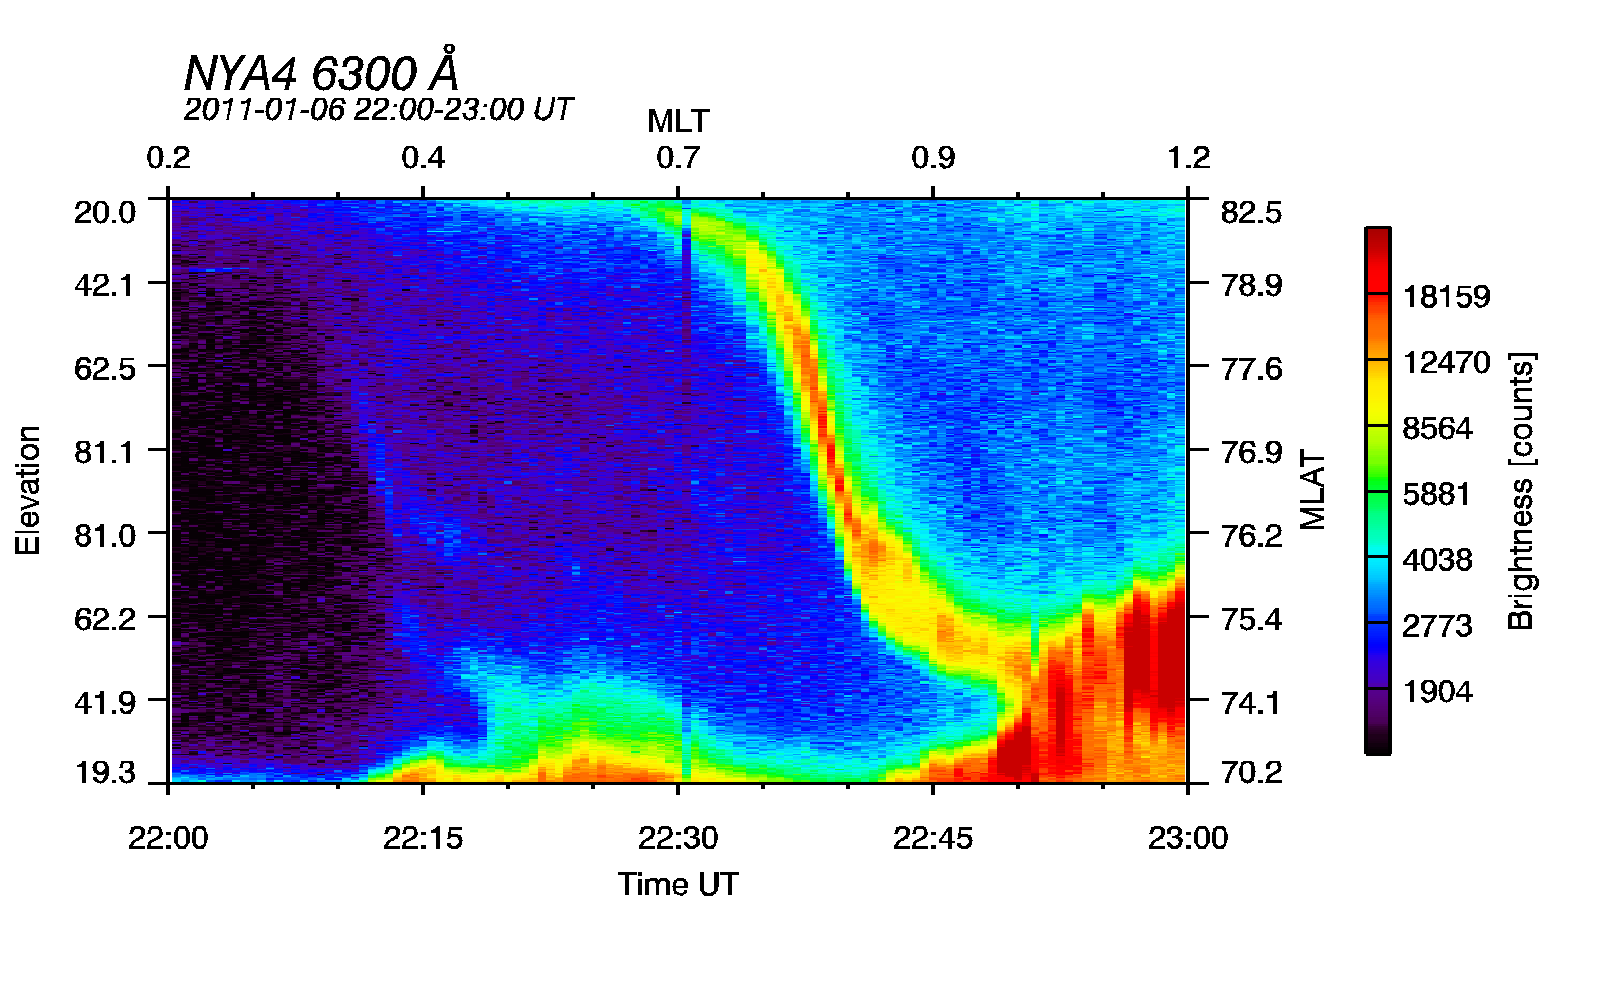
\includegraphics[width=.8\linewidth]{am-2223-6300.png}
		\caption{22-23 UT, 6300 Å}
		\label{fig:sfig6}
	\end{subfigure}
	\begin{subfigure}{.5\textwidth}
		\centering
		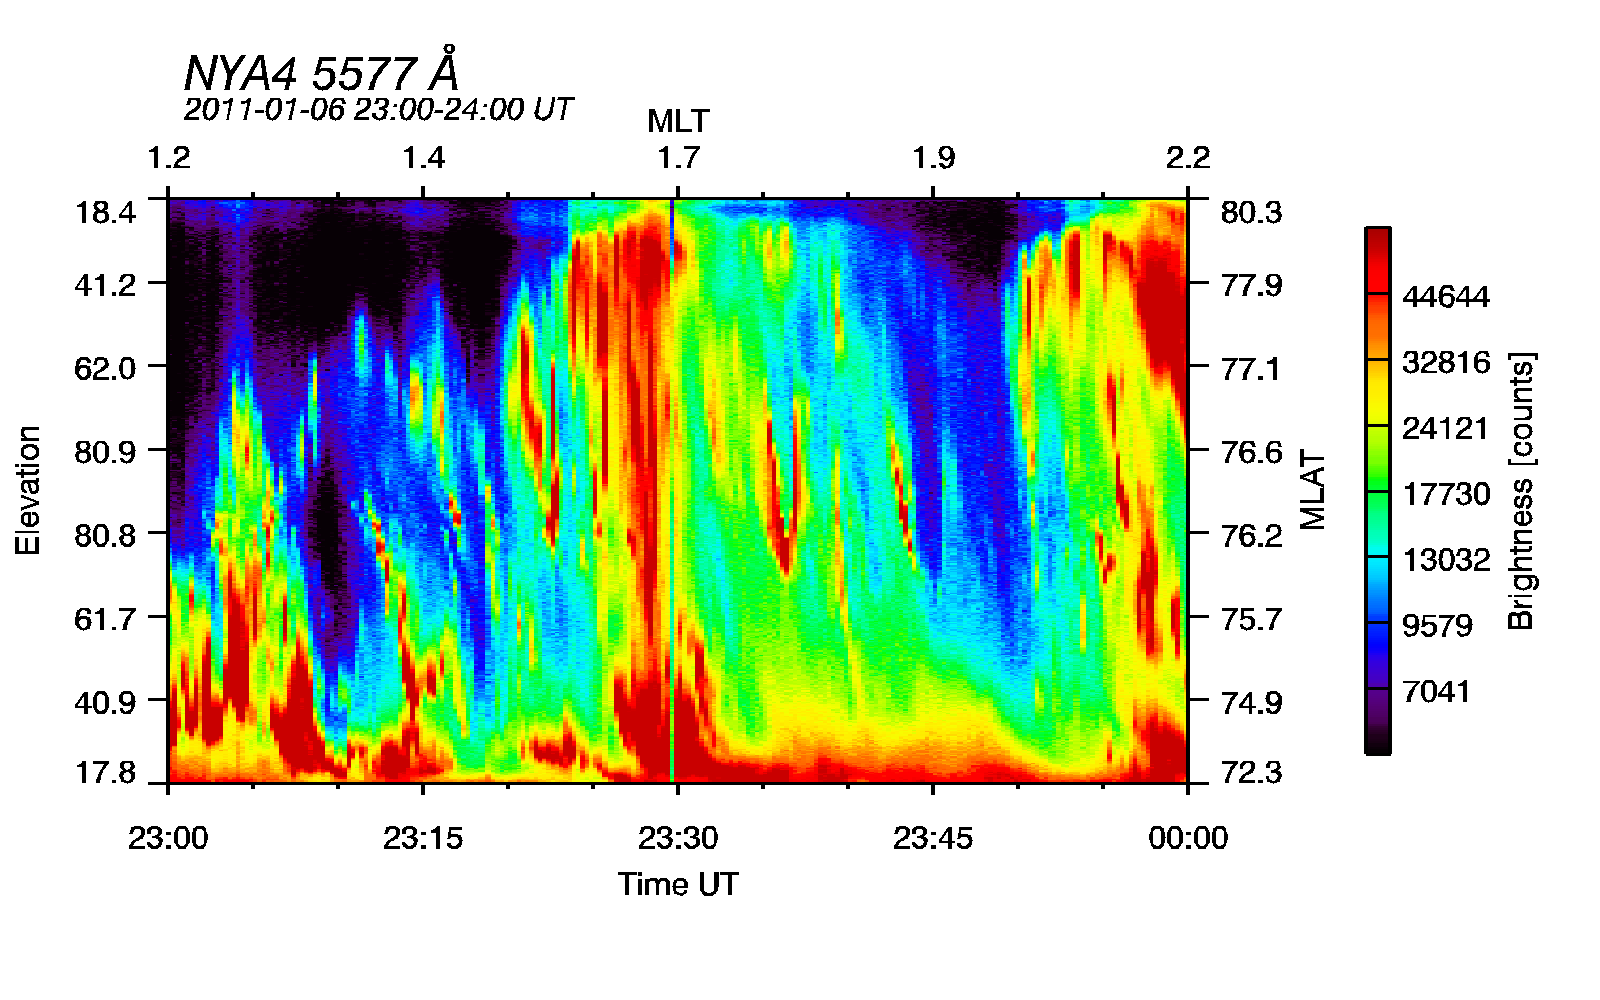
\includegraphics[width=.8\linewidth]{am-2324-5577.png}
		\caption{23-24 UT, 5577 Å}
		\label{fig:sfig7}
	\end{subfigure}
	\begin{subfigure}{.5\textwidth}
		\centering
		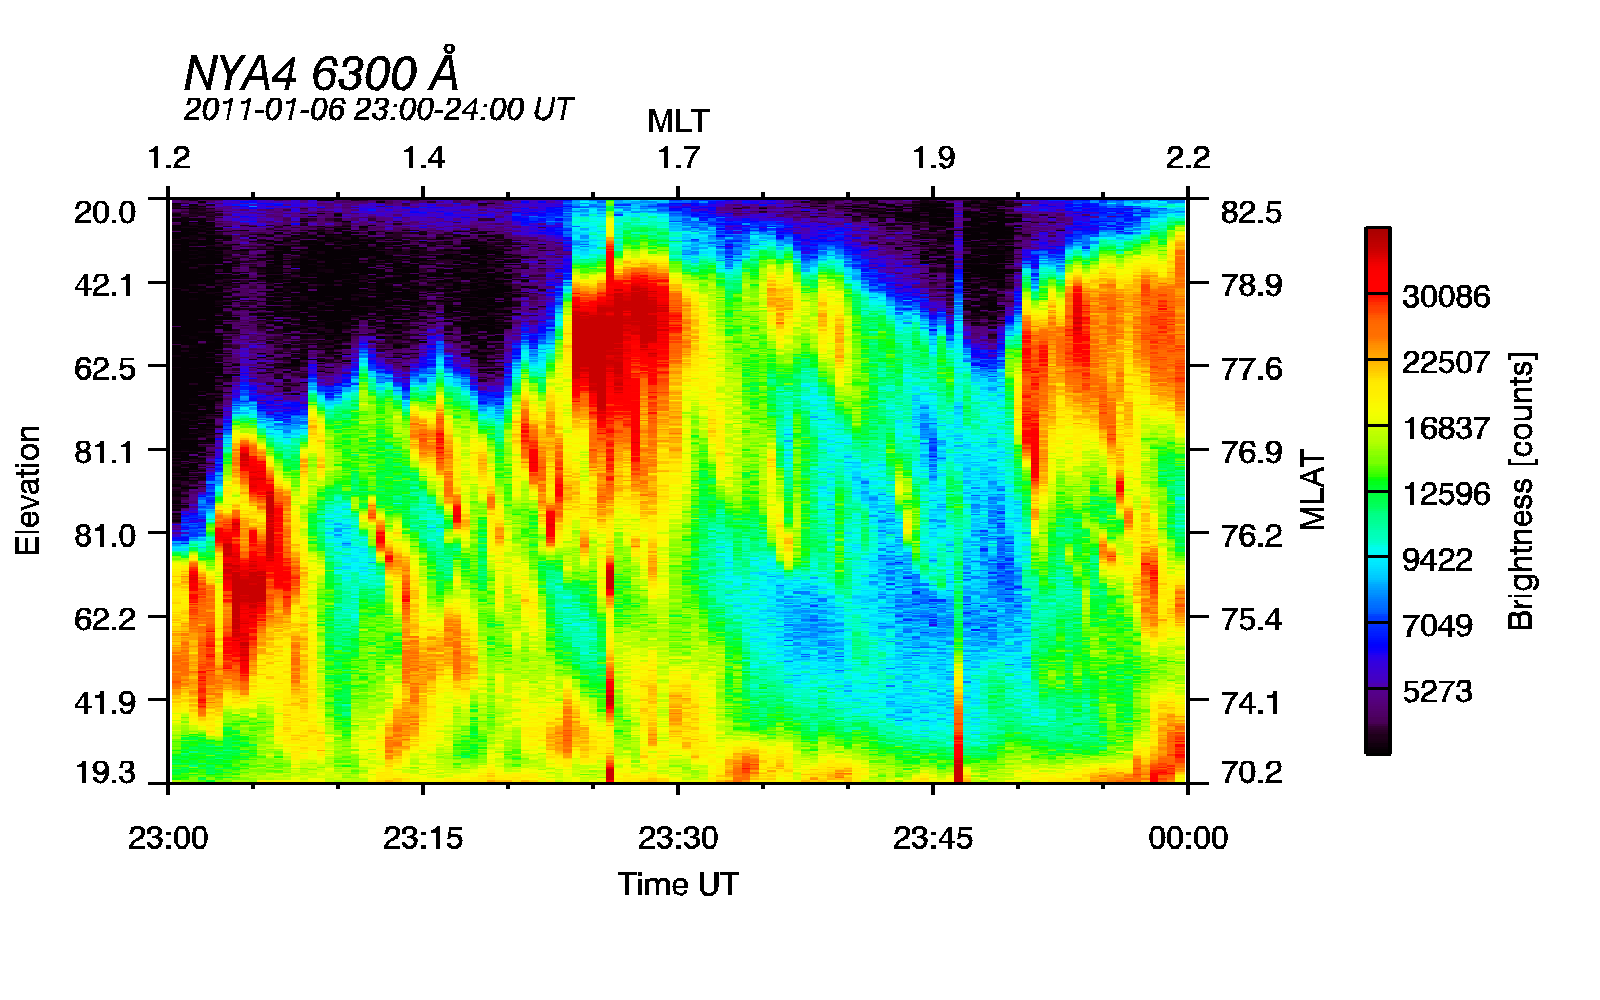
\includegraphics[width=.8\linewidth]{am-2324-6300.png}
		\caption{23-24 UT, 6300 Å}
		\label{fig:sfig8}
	\end{subfigure}
	\caption{Keograms of the All-sky camera for different times and wavelengths }
	\label{fig:fig}
\end{figure}

\begin{figure}
\begin{subfigure}{.5\textwidth}
	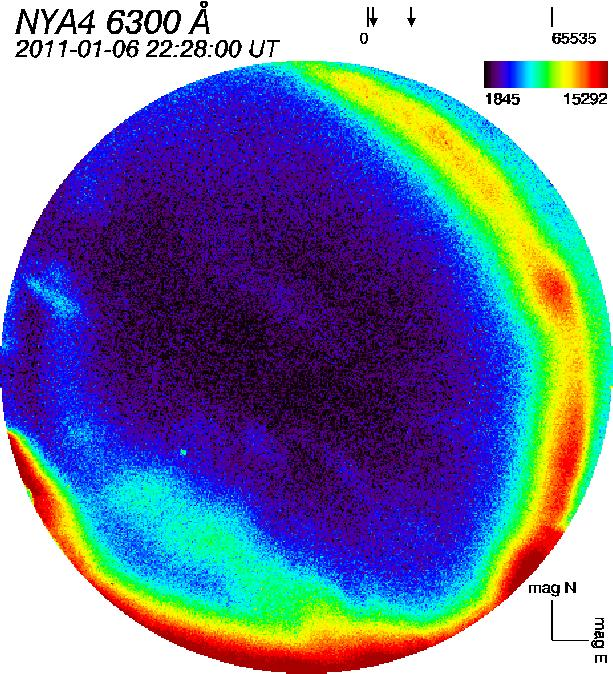
\includegraphics[width=.8\linewidth]{ame-2228-6300.jpg}
	\centering
	\caption{22:28 UT, $\lambda$ = 6300 Å}
	\label{i1}
\end{subfigure}
\begin{subfigure}{.5\textwidth}
	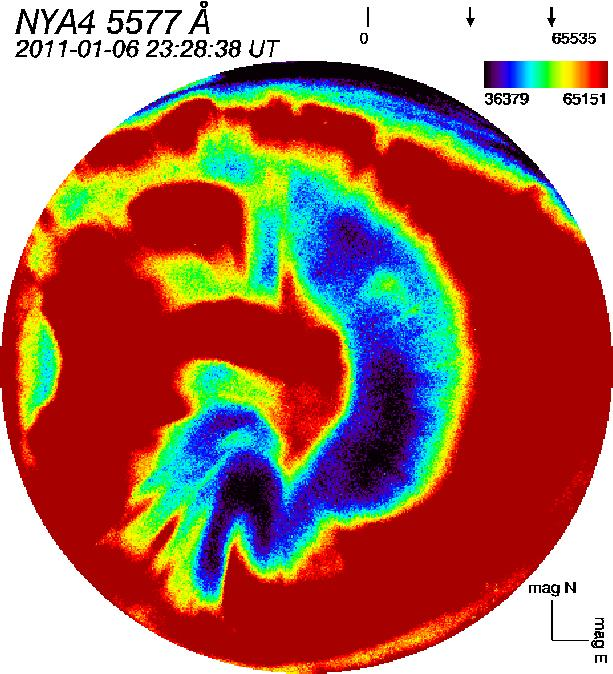
\includegraphics[width=.8\linewidth]{ame-2328-5577.jpg}
	\centering
	\caption{23:28 UT, $\lambda$ = 5577 Å}
	\label{i2}
\end{subfigure}
\caption{Images of the All-sky camera}
\end{figure}


\subsection{ACE}

I figure \ref{ace1} the components of the magnetic field of the solar wind can be seen in the timespan 17:00-23:10 UT. In the coordinate system, we are using, the geocentric solar magnetospheric system (GSM), it only depends on the z-component of the magnetic field, if magnetic reconnection at the magnetopause is possible. Is the z-component of the magnetic field of the solar wind larger than zero, then it has the opposite sign than the terrestrial magnetic field. Thus magnetic reconnection is possible. 

It can be observed, that between 17:00 and 20:10 UT, most of the time $B_Z$ is bigger than zero, but not bigger than $10 nT$. At 20:10 UT $B_Z$ drops more than $20 nT$ and then stays negative nearly all the time. Just at 22:00 UT and around 21:20 UT it goes positive. The peak at 22:00 UT is very short and just goes up to $3 nT$ while the other peak is the biggest in the entire timespan we observed. There $B_Z$ goes up to $15 nT$ and stays at this value for circa 9 minutes. Hence magnetic reconnection can happen, when this part of the solar wind reaches the magnetosphere.

In our coordinate system, the x-axis is parallel to the connection line of earth and sun. Thus we only need to look at the solar wind velocity in x-direction to calculate, how long the wind need from the satellite to earth.
In the timespan 17:00-20:00 UT the velocity $v_x$ of the solar wind is approximately constant at $v_x = 350 \frac{km}{s}$ (figure \ref{ace3}). In this time the distance between satellite and earth, $s_x$, is between $1,4509 \cdot 10^6 km$ and $1,4512 \cdot 10^6 km$. Thus the solar wind need $t = \frac{1,4510 \cdot 10^6 km}{350 \frac{km}{s}} = 69 min$ to the earth. Because the All-sky camera measures nearly no aurora before 22:00 UT, we can exclude that the solar wind at the ACE in the timespan 17:00-20:00 UT triggered the substorm.

At figure \ref{ace2} and \ref{ace4} the magnetic field components and the velocity of the solar  wind at the ACE and the position of the ACE in the time span 21:15-21:30 UT can be seen. This is the timespan, in which $B_Z$ of the solar wind peaks up to $15 nT$ and stays at this value between 21:19 UT and 21:28 UT. During the time the solar wind velocity $v_x$ is in the region $435 \frac{km}{s}-455 \frac{km}{s}$ and the distance between satellite and earth is $1.451366 \cdot 10^6 km - 1.451380 \cdot 10^6 km$. By taking the smallest distance of the satellite to earth and the biggest velocity $v_x$ in this timespan, we calculate the shortest time, the solar wind would need to earth, with the approximation that the solar wind velocity stays the same between satellite and earth. This time is $t_{min} = \frac{1.451366 \cdot 10^6 km}{455 \frac{km}{s}} = 53 min$. Thus the longest time the solar wind would need to the earth is $t_{max} = \frac{1.451380 \cdot 10^6 km}{435 \frac{km}{s}} = 56 min$. Hence the solar wind of this peak reaches the earth in the time range 22:12-22:26 UT.

As seen on the All-sky camera, the growth phase of the substorm begins around 22:20 UT when the auroral arc moves southward. This is exactly at the time, when the solar wind with a high positive $B_z$ value reaches the earth. Hence it is presumable ,that this part of the solar wind triggered the growth phase of the substorm. It interacted with the terrestrial magnetic field trough magnetic reconnection, causing the dayside reconnection to dominate. As a consequence there was a lot magnetic flux into the tail of the earth, making the tail unstable and causing the substorm's expansion phase.







\begin{figure}[h]
	\begin{subfigure}[h]{.5\textwidth}
		\centering
		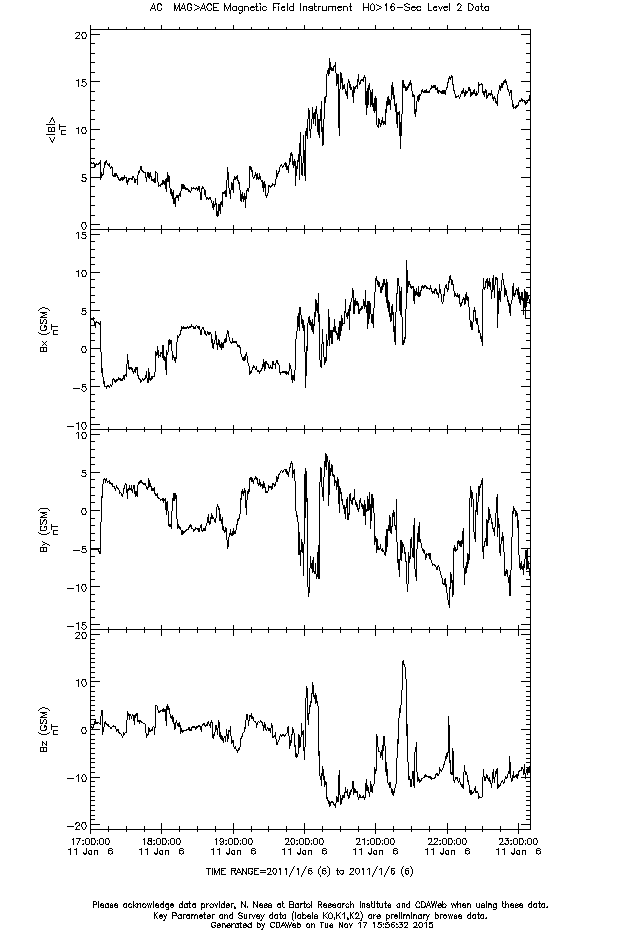
\includegraphics[width=.8\linewidth]{ace-17-2310-b.png}
		\caption{Magnetic field of the solar wind, 17:00-23:10 UT}
		\label{ace1}
	\end{subfigure}
	\begin{subfigure}[h]{.5\textwidth}
		\centering
		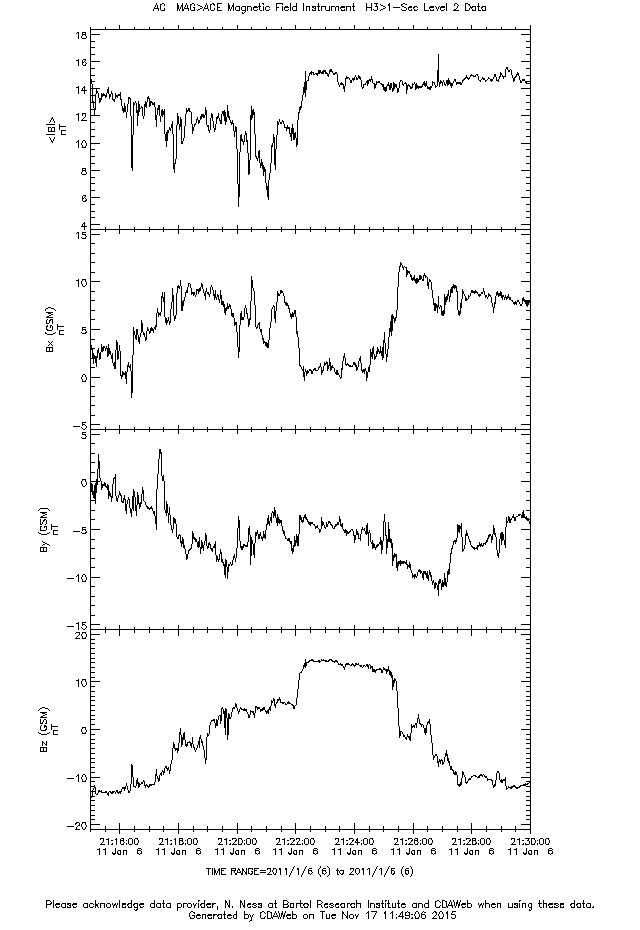
\includegraphics[width=.8\linewidth]{ace-2115-2130-b.png}
		\caption{Magnetic field of the solar wind, 21:15-21:30 UT}
		\label{ace2}
	\end{subfigure}
	\begin{subfigure}[h]{.5\textwidth}
		\centering
		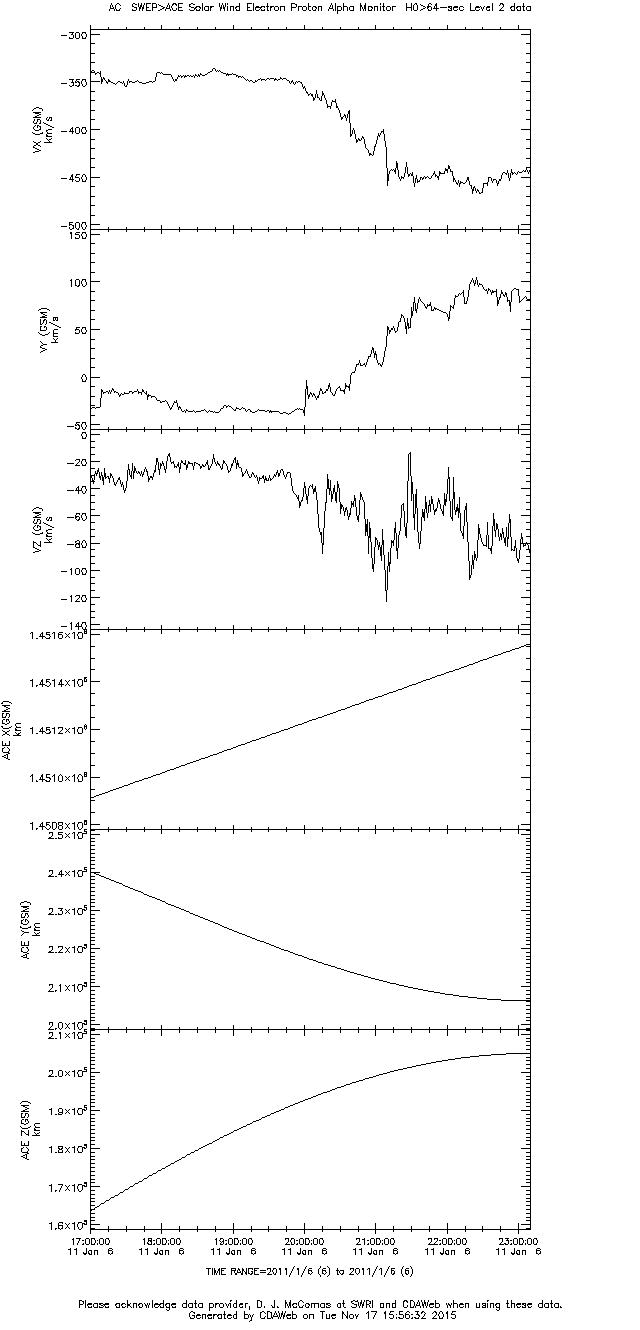
\includegraphics[width=.8\linewidth]{ace-17-2310-v-s.png}
		\caption{Velocity of the solar wind and position of the satellite, 17:00-23:10 UT}
		\label{ace3}
	\end{subfigure}
	\begin{subfigure}[h]{.5\textwidth}
		\centering
		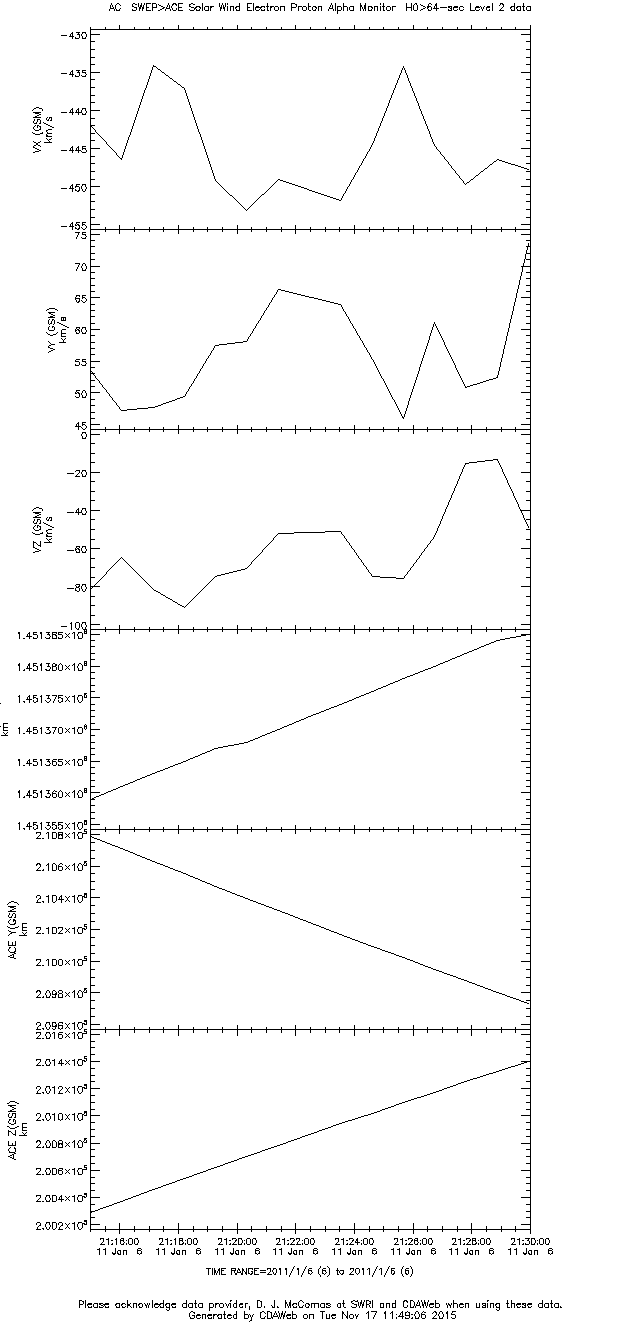
\includegraphics[width=.8\linewidth]{ace-2115-2130-v-s.png}
		\caption{Velocity of the solar wind and position of the satellite, 21:15-21:30 UT}
		\label{ace4}
	\end{subfigure}
	\caption{Measurements of the ACE}
	\label{ace}
\end{figure}







\section{Sources}

Websites:

	\url{http://tid.uio.no/plasma/aurora/tech.html}
	
	\url{https://en.wikipedia.org/wiki/Advanced_Composition_Explorer}
	
	\url{https://en.wikipedia.org/wiki/Super_Dual_Auroral_Radar_Network}
	
	\url{https://en.wikipedia.org/wiki/Iridium_satellite_constellation}
	
	\url{http://www.jhuapl.edu/newscenter/pressreleases/2010/100818.asp}
	
	\url{https://directory.eoportal.org/web/eoportal/satellite-missions/a/ampere}
	
Graphics:

	\url{http://tid.uio.no/plasma/aurora/data.php}
	
	\url{http://vt.superdarn.org/tiki-index.php?page=radarFoV}


\end{document}